
% plantilla obtenida de: https://www.overleaf.com/19886281jjqffwsxshmm#/73112823/

\documentclass[a4paper, 11pt]{article}
\usepackage{comment} % enables the use of multi-line comments (\ifx \fi) 
\usepackage{lipsum} %This package just generates Lorem Ipsum filler text. 
\usepackage{fullpage} % changes the margin

\usepackage[spanish]{babel}
\usepackage[utf8]{inputenc}

\usepackage{graphicx}

\usepackage{amsmath}
\usepackage{amsfonts}
% or
\usepackage{amssymb}
\usepackage{tikz}
\usepackage{array}
\newcolumntype{C}{>{$}l<{$}} % math-mode version of "l" column type
\newcommand{\imageins}[4]{\begin{figure}[!ht]		%Take the hardwork from using images. Let this command do the work for you. Insert images by just using this command \imageins{filename}{width as a ratio of total text width of the page}{caption name}{label name for referring in articles}		
    \centering
    \includegraphics[width=#2\textwidth]{#1}
    %\caption{#3}
    %\label{#4}
    \vspace{0.2em}
\end{figure}}

%%%%%%%%%%%%%%%%%%%%%%%%%%%%%%%%%%%%%%%%%%%%%%%%%%%%%%%%%%%%%%%%%%%%%%%%%%%%%%%%%%
\usepackage{listings}
\usepackage{color}
 
\definecolor{codegreen}{rgb}{0,0.6,0}
\definecolor{codegray}{rgb}{0.5,0.5,0.5}
\definecolor{codepurple}{rgb}{0.58,0,0.82}
\definecolor{backcolour}{rgb}{0.95,0.95,0.92}
 
\lstdefinestyle{mystyle}{
    backgroundcolor=\color{backcolour},   
    commentstyle=\color{codegreen},
    keywordstyle=\color{magenta},
    numberstyle=\tiny\color{codegray},
    stringstyle=\color{codepurple},
    basicstyle=\footnotesize,
    breakatwhitespace=false,         
    breaklines=true,                 
    captionpos=b,                    
    keepspaces=true,                 
    numbers=left,                    
    numbersep=5pt,                  
    showspaces=false,                
    showstringspaces=false,
    showtabs=false,                  
    tabsize=2
}
 
\lstset{style=mystyle}

%%%%%%%%%%%%%%%%%%%%%%%%%%%%%%%%%%%%%%%%%%%%%%%%%%%%%%%%%%%%%%%%%%%%%%%%%%%%%%%%%%

\begin{document}
%Header-Make sure you update this information!!!!
\noindent
\large\textbf{Práctica II} \hfill \textbf{Antonio Gámiz Delgado} \\
\normalsize Fundamentos de Redes \hfill 10/11/2018
%\normalsize ECE 100-003 \hfill Teammates: Student1, Student2 \\
%Prof. Oruklu \hfill Lab Date: XX/XX/XX \\
%TA: Adam Sumner \hfill Due Date: XX/XX/XX

\section{Descripción.}

Para esta práctica he hecho una aplicación que da un servicio de \textit{login} y \textit{broadcasting}. El objetivo de la misma es permitir al cliente que se registre e inicie sesión con un \textit{usuario} y \textit{contraseña} definidos por él. Una vez haya iniciado sesión, al cliente se la pregunta por un tiempo de conexión, en milisegundos. Ese dato indica durante cuanto tiempo estará recibiendo datos, y una vez pasado ese tiempo, se procederá a la desconexión y cierre de la conexión.

Para implementar esta aplicación, he creado un nuevo protocolo usando como base TCP. Los elementos de este protocolo pueden encontrarse en el archivo \textit{Protocolo.java}. Clase creada para almacenar los códigos de los distintos paquetes, así como dos métodos para recibir y emitir paquetes, para hacer el código de la aplicación más simple y entendible. 

El servidor es concurrente, cada vez que llega una nueva conexión se lanza una nueva hebra (instancia de la clase \textit{User} (\textit{User.java}), que se encarga de identificar al cliente ( método \textit{identify()} y de efectuar la posterior desconexión del mismo. 

Al inicializar el servidor, se crea una nueva hebra, instancia de la clase \textit{Transmitter} (\textit{Transmitter.java}), que se encarga de hacer el \textit{broadcasting} de los datos a todos los clientes conectados a través de un \textit{ArrayList\textless User\textgreater} que mantiene el Server con todas los usuarios conectados en ese momento.
 
\section{Diagrama de estados del servidor.}

\begin{figure}[h]
\center
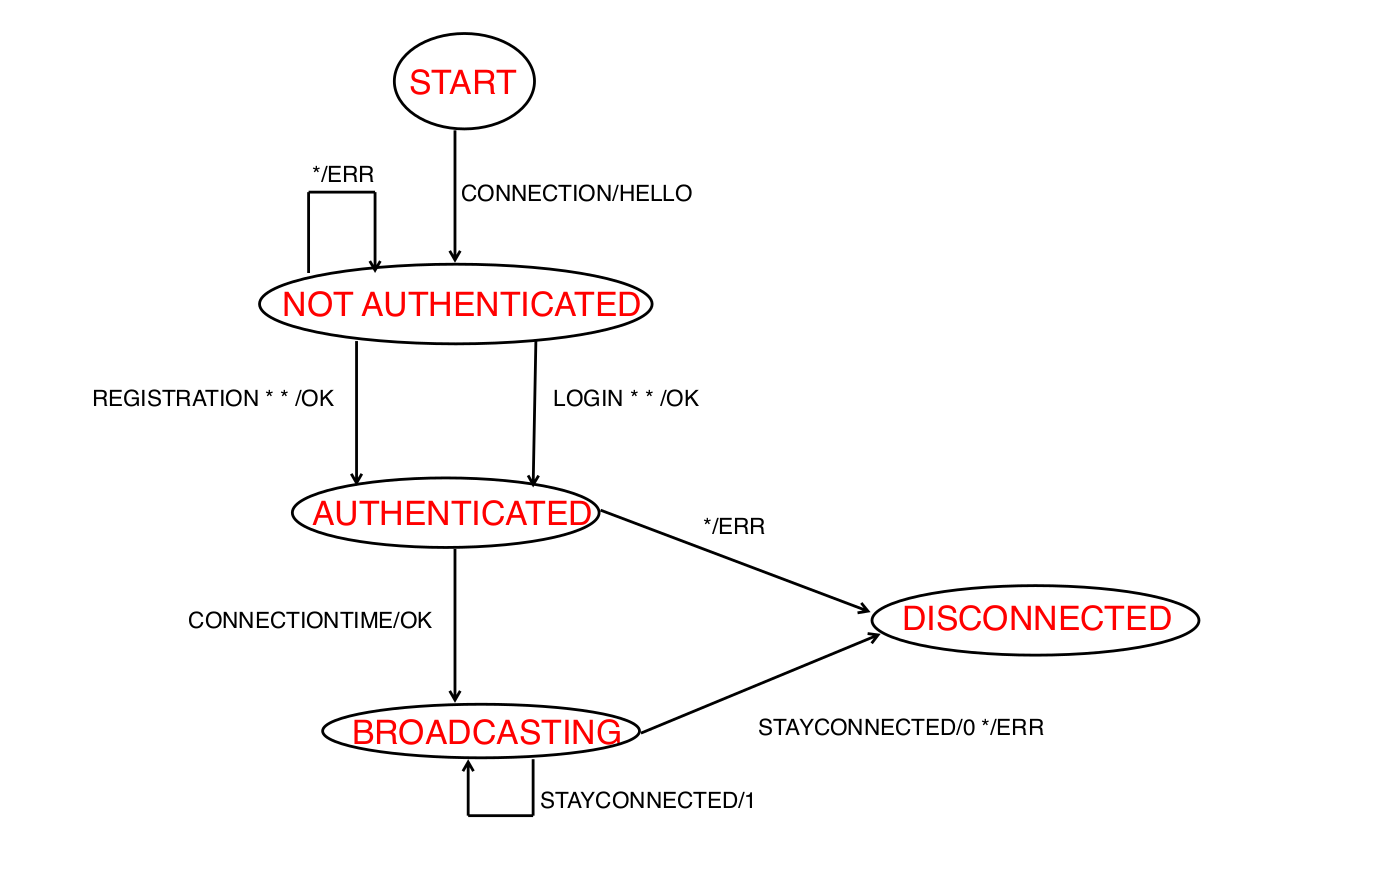
\includegraphics[scale=0.70]{diagram.png}
\end{figure}

\section{Mensajes que intervienen}
\begin{figure}[h]
\center
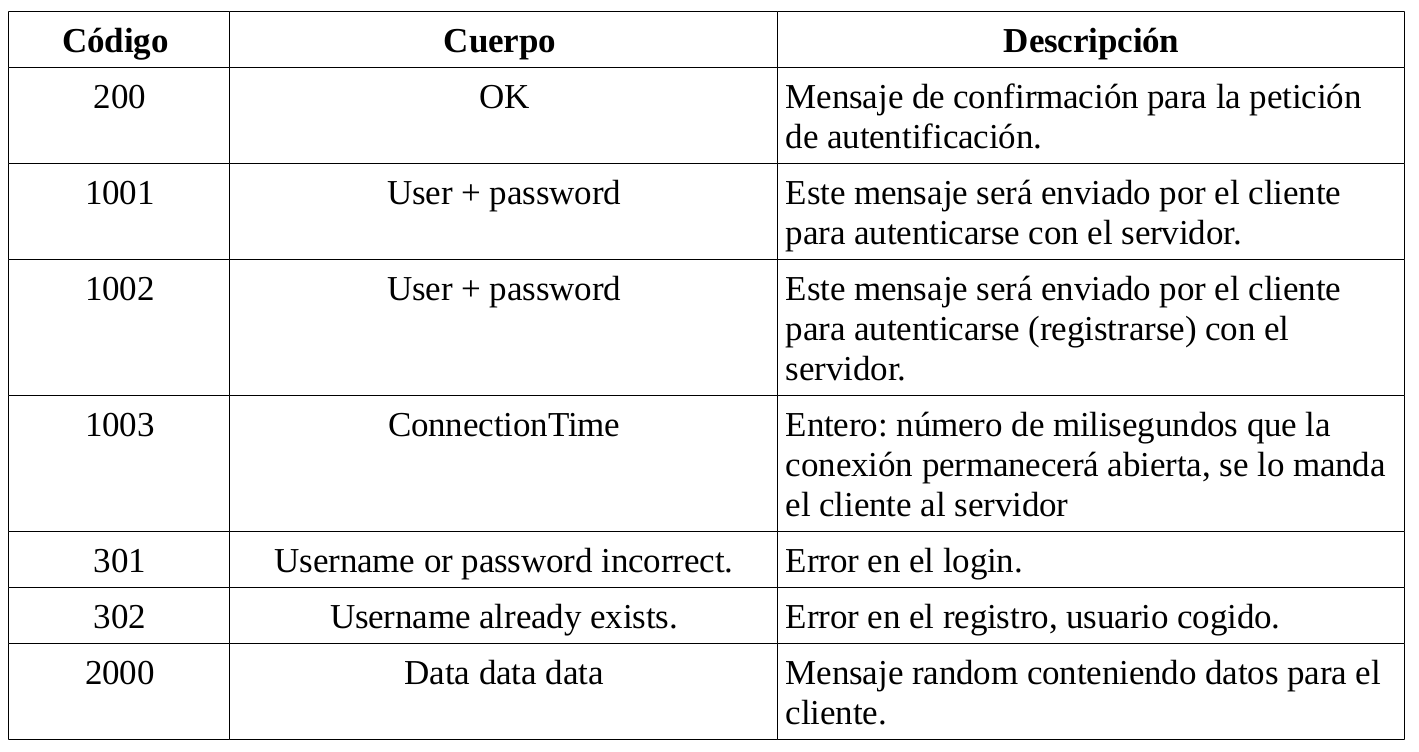
\includegraphics[scale=0.3]{codes.png}
\end{figure}
\
\section{Evaluación de la aplicación.}

\begin{figure}[h]
\center
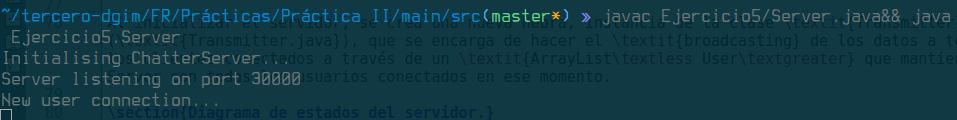
\includegraphics[scale=0.5]{1.png}
\caption{Inicialización del servidor.}
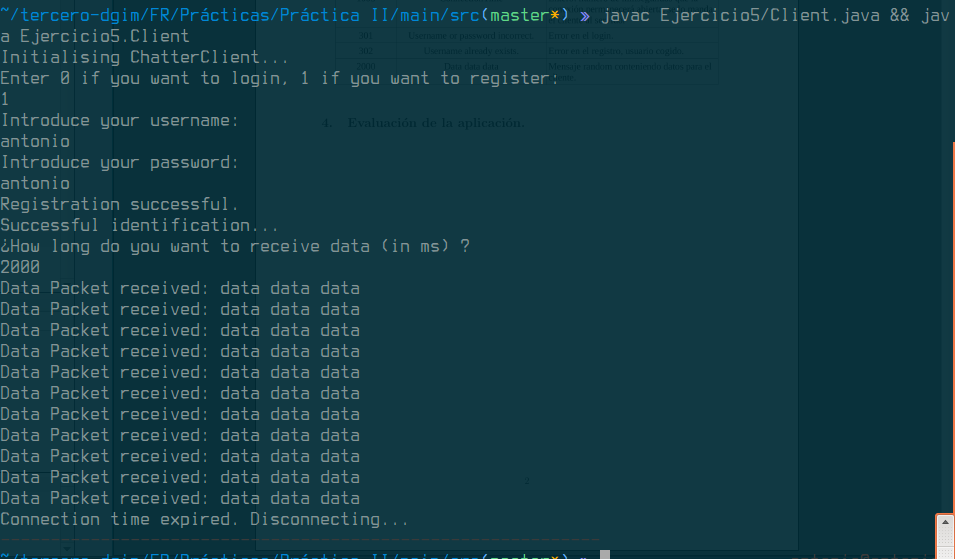
\includegraphics[scale=0.4]{3.png}
\caption{Nos registramos y empezamos a recibir datos, y se corta la conexión.}
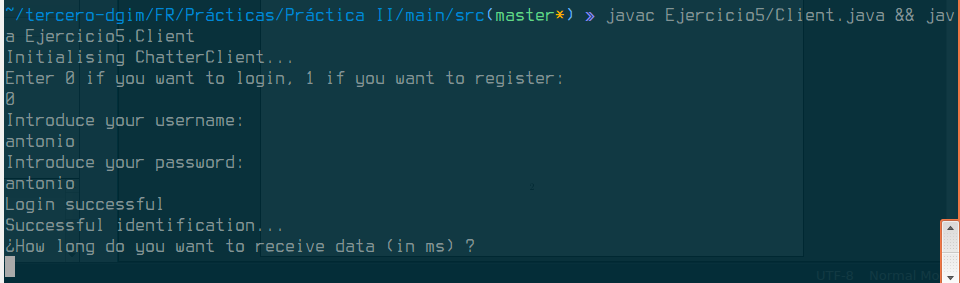
\includegraphics[scale=0.4]{4.png}
\caption{Nos logeamos otra vez con el usuario creado.}
\end{figure}
\newpage
\begin{figure}[t]
\center
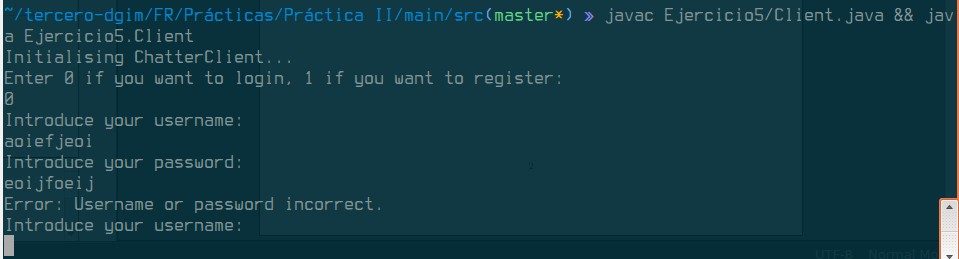
\includegraphics[scale=0.45]{5.png}
\caption{Intetamos logearnos con un usuairo inexistente.}
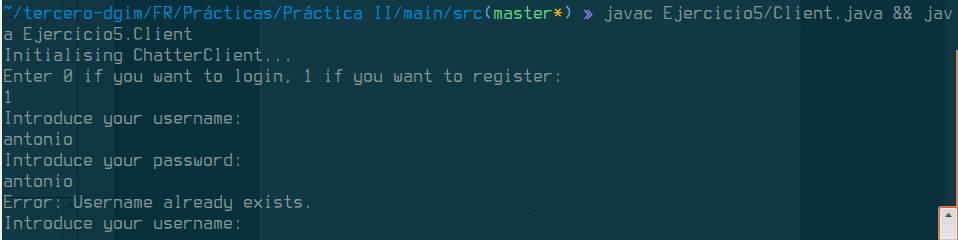
\includegraphics[scale=0.45]{6.png}
\caption{Intentamos registrarnos con un usario ya existente.}

\end{figure}

\end{document}